\documentclass[../../lecture_notes.tex]{subfiles}
\begin{document}


The original NFS assumed both the client and server kernels are trustworthy and that the server UID’s match with the client UID’s.

How does NFS address the superuser? (obviously every root can’t have root permissions)
\begin{itemize}
\item we make user 0 “nobody” and give them minimal privileges
\end{itemize}
This is simplistic: the naming scheme in reality is complicated and involves strings.

Soon after, we developed authentication (via Kerberos, etc) to encrypt packets. We need this authentication to prevent attacks against:
\begin{enumerate}[nosep]
\item Privacy (unauthorized release of information)
\item Integrity (tempering with unauthorized data)
\item Service (Denial of Service)
\end{enumerate}


Our goals are therefore:
\begin{itemize}
\item Allow authorized access (+)
\item Disallow unauthorized access (-)
\item Good performance (+)
\end{itemize}
Positive goals are easy because they get reported, but negative goals are more difficult


When attempting to build a secure system, we perform \term{Threat Modeling}; the threats to the security of a system include:
\begin{itemize}
\item insiders
\item social engineering (generally non-coding)
\item network attacks (virus, DOS)
\item device attacks (USB) attacks
\end{itemize}
The last is so common that it is recommended people use a "usb condom".


Our security within a system is trivial; we simply chroot untrusted processes so they think they have access to the root. Even this is not perfect, however: for instance, processes P and P’ can communicate with gettimeofday(), where P chews up computer time and P’ checks the clock, transmitting data with only clock change. In this way, P can send messages using morse code. This is called a \term{covert channel}, and they are effectively unavoidable; we instead only focus on critical attacks


To prevent these, our system requires 4 major properties
\begin{enumerate}[nosep]
\item Authentication (password, credentials)
\item Integrity (checksum)
\item Authorization (access control list)
\item Auditing (log)
\end{enumerate}
and obviously correctness and performance.


\subsection{Authentication}

We utilize \term{authentication} to prevent masquerading. Authentication is based on 3 major properties:
\begin{enumerate}[nosep]
\item who the principal is (ex. retinal scan)
\item something the principal has (ex. smart card)
\item something the principal knows (ex. password)
\end{enumerate}
but these are often equivalent, as we can bootstrap from one to the other. For example, SEASNET is based on (1) but uses (3) for verification.


There are two phases of authentication:
\begin{enumerate}
\item \term{external authentication} $\coloneqq$ protection from the outside world.
\begin{itemize}
	\item the system verifies that the user is a part of the system
	\item examples include a trusted login agent (OS), key, password, biometrics, MFA
	\item attack types
		\begin{itemize}
			\item theft of hardware tokens
			\item fraudulent servers
			\item chain breaking
			\item buggy login agents
			\item well known default passwords
			\item SIN attacks (SIM card backup)
			\item password recovery attacks
			\item bad routers
		\end{itemize}
	\item From an OS standpoint, many of these are beyond our purview.
\end{itemize}

\item \term{internal authentification} $\coloneqq$ protection from inside the system
\begin{itemize}
	\item the system verifies the user is a specific member of a system
	\item by design, internal authentification is much more efficient
	\item common type of attack is a PATH injection:
		\begin{itemize}
			\item Internal authentication in Linux comes in the form of UIDs
			\item The UID is the current user, and the EUID is the program’s creator
			\item There are select programs (called setuid programs) which this is not true for; these are marked with a UID execution bit of “s”
			\item These programs are automatically trusted by the root (ex. /usr/bin/passwd)
			\item a PATH injection is a bad user setting the path such that a system() call behaves poorly
			\item For that reason, we avoid usages such as system(“ls”)
		\end{itemize}
\end{itemize}
\end{enumerate}

\begin{center}
\begin{tikzpicture}
\node[align=center] (setreuid) {superuser\\\texttt{setreuid}(\textit{ruid}, \textit{euid})};
\node[right=3cm of setreuid, align=center] (setuid) {superuser\\\texttt{setuid}(\textit{uid})};
\node[right=3cm of setuid, align=center] (seteuid) {superuser\\\texttt{seteuid}(\textit{uid})};
\node[below=2cm of setreuid, rectangle, minimum width=2cm, minimum height=1cm, draw, 
	align=center] (reuid) {real\\user ID};
\node[below=2cm of setuid, rectangle, minimum width=2cm, minimum height=1cm, draw, 
	align=center] (uid) {effective\\user ID};
\node[below=2cm of seteuid, rectangle, minimum width=2cm, minimum height=1cm, draw, 
	align=center] (euid) {saved\\set-user-ID};
\draw[-Latex] (setreuid) -- node[pos=0.5, left] {\scriptsize\textit{ruid}} (reuid);
\draw[-Latex] (setuid) -- node[pos=0.5, right] {\scriptsize\textit{uid}} (uid);
\draw[-Latex] (setreuid) -- node[pos=0.25, above right, rotate=-30] {\scriptsize\textit{euid}} (uid);
\draw[-Latex] (setuid) -- node[pos=0.25, above left, rotate=30] {\scriptsize\textit{uid}} (reuid);
\draw[-Latex] (setuid) -- node[pos=0.25, above right, rotate=-30] {\scriptsize\textit{uid}} (euid);
\draw[-Latex] (seteuid) -- node[pos=0.25, above left, rotate=30] {\scriptsize\textit{uid}} (uid);
\draw[-Latex] (reuid) to [out=285, in=255] node[below, pos=0.5, align=center] 
	{unprivelaged\\\texttt{setuid} or \texttt{seteuid}} (uid);
\draw[-Latex] (euid) to [out=255, in=285] node[below, pos=0.5, align=center] 
	{unprivelaged\\\texttt{setuid} or \texttt{seteuid}} (uid);
\draw[-Latex] (reuid) to [out=15, in=165] node[pos=0.5, below, align=center] {unprivelaged\\\texttt{setreuid}} (uid);
\draw[-Latex] (uid) to [out=195, in=-15] (reuid);
\draw[-Latex] (euid) to [out=165, in=15] node[pos=0.5, below, align=center] {unprivelaged\\\texttt{setreuid}} (uid);
\node[below left=0cm and 0.7cm of euid, align=center] (exec) {\texttt{exec} of\\set-user-ID};
\draw[-Latex] (exec) -- (uid);\draw[-Latex] (exec) -- (euid);
\end{tikzpicture}
\end{center}


Shells are at risk for PATH injection, since they implicitly call system(), but our c programs must be reliable (especially in terms of buffer overflow). Sometimes, however, there isn’t much we can do (take setuid()). At least setuid() requires root access

Once we verify identity, we move on to:

\subsection{Authorization}

There are two schemes for access to resources:
\begin{enumerate}
\item \term{Direct Access}
\begin{lstlisting}
char *p = mmap(fd, offset, etc...);
\end{lstlisting}
	The system checks authority once and maps a pointer onto the process address space. Thus is done with page table manipulation.
	Properties: \begin{enumerate}[nosep]
		\item[+] high performance
		\item[-] easy resource corruption (by bad actors and race conditions)
		\item[-] necessitates hardware support
	\end{enumerate}

\item \term{Indirect Access}
\begin{lstlisting}
int fd = open(file, ...);
read(fd, ...);
\end{lstlisting}
The system issues a request to handler or system call to check on every attempted resource access.
\begin{enumerate}[nosep]
\item[-] low performance
\item[+] avoid corruption
\item[+] easier to revoke permission
\end{enumerate}
\end{enumerate}

We can think of an operating system as a set of principals and resources:

\begin{minipage}{0.4\linewidth}
\centering
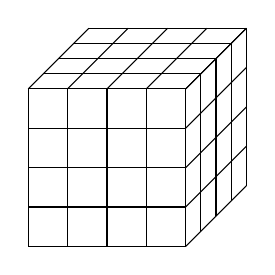
\begin{tikzpicture}[scale=0.5]
\foreach \x in{0,...,4}
{   \draw (0,\x ,4) -- (4,\x ,4);
    \draw (\x ,0,4) -- (\x ,4,4);
    \draw (4,\x ,4) -- (4,\x ,0);
    \draw (\x ,4,4) -- (\x ,4,0);
    \draw (4,0,\x ) -- (4,4,\x );
    \draw (0,4,\x ) -- (4,4,\x );
}
\end{tikzpicture}
\end{minipage}%
\begin{minipage}{0.6\linewidth}
\begin{itemize}
\item We require 3 parameters to check whether a given user can access a given resource.
\item This array seems massive, but the data is not random, so there must be a more efficient way to represent the information.
\end{itemize}
It turns out we can represent it in two dimensions!
\end{minipage}


We do this with an \term{Access Control List}
\begin{lstlisting}[language=sh]
$ getfacl .
user: rwx
group: r-x
other: r-x
$ setfacl -m g:tas:rwx .
$ getfacl .
user: rwx
group: r-x
other: r-x
tas: rwx
# we have appended the group "tas" to the end of the directory's list
\end{lstlisting}

Associated with each file is a list of access rights under the control of the file’s owner. Using this, we can form our own ad-hoc groups outside of the built-in ones.

This is not the only way to represent authorization, and isn’t perfect for every purpose; we may need to capturing rights accurately or letting ordinary users specify rights. ACLs in general are not flexible enough for large organizations. Instead we can use role-based access control (RBAC); this model more complex but secure than ACLs.

The model: keep a distinction between users and their roles. 

For example, the user "eggert" could have multiple roles assigned to him: ie eggert as cs-faculty and as sys-admin
\begin{itemize}
\item cs-faculty allows him to change grades. 
\item sys-admin allows him to make changes to other users' permissions.
\end{itemize}
These permissions are usually mutually exclusive, and roles can have sub-roles, which may share some permissions.

In both models, each file lists permissions for each user; these are \term{resource-centric}. We can instead use a principal-centric model called a \term{Capability Model}, where users hold an object with an unforgeable unique ID representing a resource.
    

Linux utilizes both approaches
\begin{itemize}
\item Each descriptor has its own separate permissions from the file (capability)
\item Each file is resource-centric and holds its own permissions
\end{itemize}
\begin{lstlisting}
fd = open ("abc", O_RDONLY)             <--- code
r--              rwx                    <--- permissions
read-only        read, write, execute   <--- description of permissions
// the file "abc" has the permissions rwx
// the fd is the capability with permissions r--
// any action done with fd can only read, even though the file is rwx
\end{lstlisting}

Note that the flags could include O\_PATH, which gives no permissions, only showing the existence of the file. We could then duplicate the file descriptor using dup2, but then you'd have 2 useless fd's.

We can therefore run:
\begin{lstlisting}
int stat(const char *path, struct stat *buf);
// return information about the file that fd points to
\end{lstlisting}

We have addressed \term{auditing} with logs and \term{integrity} with checksums already.


\end{document}